\def\CTeXPreproc{Created by ctex v0.2.9, don't edit!}
%\documentclass{beamer}
\documentclass[%handout,
xcolor=pdftex]{beamer}
\mode<presentation> {
  \usetheme{Warsaw}
  \setbeamercovered{transparent}
}
\let\Tiny=\tiny
\usetheme{Singapore}
\usecolortheme{dolphin}
\usepackage{amsmath}
\usepackage{textcomp}
\usepackage{amssymb}
\usepackage{amsthm}
\usepackage{graphicx}
\usepackage{color}
\usepackage{lipsum}
\usepackage{hyperref}
\usepackage{multirow}
\usepackage{bm}
%\setbeamertemplate{headline}{}
\setbeamertemplate{footline}[page number]
\newcommand\Fontvi{\fontsize{9pt}{8}\selectfont}
\newcommand\Fontvii{\fontsize{7pt}{8}\selectfont}
\newcommand{\backupbegin}{
   \newcounter{finalframe}
   \setcounter{finalframe}{\value{framenumber}}
}
\newcommand{\backupend}{
   \setcounter{framenumber}{\value{finalframe}}
}\newtheorem{proposition}{Proposition}
\title{Unit 8: ARMA Models: AR(1)}
\author[STAT 5170: Applied Time Series, Unit 8]{Jeffrey Woo}
\institute{Department of Statistics, University of Virginia}
\date{Spring 2020}

\AtBeginSubsection[] {
  \begin{frame}<beamer>{Outline}
    \tableofcontents[currentsection,currentsubsection]
  \end{frame}
}

\begin{document}


\frame{\titlepage}


\begin{frame}
\frametitle{Readings for Unit 8}

Textbook chapter 3.1 (page 75 to 79).

\end{frame}


\begin{frame}
\frametitle{So Far...}

We have mainly discussed a number of techniques in exploratory data analysis that will aid us in understanding the behavior of various time series. These should be used as a guide to help us decide what kind of model is appropriate.

\end{frame}

\begin{frame}
\frametitle{This Unit}
\begin{enumerate}
\item AR(p) process
\item AR(1) process
\item AR(1) in terms of backshift operator
\item AR(1) and causality
\end{enumerate}
\end{frame}

\begin{frame}
\frametitle{Motivation}

Next, we discuss ARMA models which is a time series where the current observation depends on a linear combination of past observations plus  a ``noise'' term which is conceivably a moving average process.  We will discuss the models and some of their properties.  We will discuss how to fit these models and how to do forecasting from the models once we fit them.  We will also discuss how to select among competing models, and then we will discuss how to handle seasonal components.

\end{frame}

\section{AR(p) Process}
\frame{\tableofcontents[currentsection]}

\begin{frame}
\frametitle{AR(p) Process}

Recall the definition of an autoregressive
process: $x_t$ is an autoregressive model of order $p$, AR(p), if it can be written as
\begin{equation} \label{eq:ar1}
x_t =\phi_1 x_{t-1} + \phi_2 x_{t-2} +...+  \phi_p x_{t-p} + w_t
\end{equation}

where $w_t$ is a Gaussian white noise process with variance $\sigma_w^2$.
\end{frame}

\begin{frame}
\frametitle{AR(p) Process}

If we would like to include a nonzero mean we can generalize the AR(p) model (\ref{eq:ar1}) as
$$
x_t-\mu =\phi_1 (x_{t-1}-\mu)+ \phi_2 (x_{t-2}-\mu)+...+  \phi_p (x_{t-p}-\mu) + w_t.
$$
You can think about this as having an AR(p) after transforming the data by removing a mean.

\end{frame}

\begin{frame}
\frametitle{AR(p) Process}

Another way to write this is
$$
x_t=\alpha+\phi_1 x_{t-1} + \phi_2 x_{t-2} +...+  \phi_p x_{t-p} + w_t
$$
where $\alpha=\mu(1-\phi_1-...-\phi_p)$.  This is closer to how one writes a regression model.  Note that $\alpha$ will NOT be the mean of $x_t$.

\end{frame}


\begin{frame}
\frametitle{Backshift Operator}

Recall the \textbf{backshift operator}.  For any $t$,
$$
B x_t =x_{t-1}.
$$
As an example we can rewrite the \textbf{differencing operator} as
$$
\nabla x_t =x_t-x_{t-1}=(1-B)x_{t}.
$$

We can also use powers of $B$ such as
$$
B^p x_t = x_{t-p}.
$$

\end{frame}

\begin{frame}
\frametitle{AR(p) Process}

So, we may rewrite the $AR(p)$ model as
\begin{eqnarray} \label{eq:ar_op}
 & =&  \nonumber \\
 & =&  \nonumber \\
 & =&     \nonumber \\
\phi(B) x_t & =&    w_t
\end{eqnarray}

where $\phi(B)=$ \\
\vspace{5mm}
This function $\phi(B)$ is called the \textbf{autoregressive operator}.  This is a ``polynomial'' in $B$.  It will be important to determine what choices of the coefficients will give us a stationary process.

\end{frame}


\section{AR(1) Process}
\frame{\tableofcontents[currentsection]}

\begin{frame}
\frametitle{AR(1) Process}

We will now look more in depth at the simplest case the $AR(1)$ process. We will discuss
$$
x_t= \phi x_{t-1}+w_t
$$
for $t=...,-1,0,1,2,...$.
We would like to clearly determine the mean, variance, and autocovariance of this process.

\end{frame}


\begin{frame}
\frametitle{AR(1) Process}

Earlier we discussed that we may use recursion to hopefully simplify this process.
\begin{eqnarray} \label{eq:recursive}
 & =&  \nonumber \\
 & =&  \nonumber \\
& =&  \nonumber \\
 &=&  \nonumber\\
&=&  \nonumber \\
...& & \nonumber \\
x_t & =&  \phi^k   x_{t-k}+\sum_{j=0}^{k-1} \phi^j w_{t-j}.
\end{eqnarray}

\end{frame}

\begin{frame}
\frametitle{AR(1) Process}

Notice that if $|\phi|<1$, then the first term in (\ref{eq:recursive}) becomes very small.  So, in fact, we can say that as $k \rightarrow \infty$ that
\begin{eqnarray} \label{eq:short}
x_t &=& \sum_{j=0}^{\infty} \phi^j w_{t-j} \nonumber \\
    &=& \sum_{j=0}^{\infty} \phi^j B^j w_t.
\end{eqnarray}
This is an $MA(\infty)$ process.

\end{frame}


\begin{frame}
\frametitle{AR(1) Process}

We next show that if $|\phi| < 1$, then an AR(1) is stationary. Note that in unit 3, we showed that if an AR(1) is stationary, then $|\phi| < 1$.\\

\vspace{5mm}

The representation in (\ref{eq:short}) should make doing things like calculating the mean easier. First of all, it should be clear that
 $$
 Ex_t =0.
 $$

\end{frame}

\begin{frame}
\frametitle{AR(1) Process}

Next, we would like to calculate the variance.

\vspace{50mm}

So, the mean and variance are constant.


\end{frame}

\begin{frame}
\frametitle{AR(1) Process}

We now need to only
verify that the covariance also does not depend on time but
only the lag. Since the mean is zero, we need to find, for
$h > 0$,

\vspace{50mm}

\end{frame}

\begin{frame}
\frametitle{AR(1) Process}

Note also, that the true $ACF$ is
$$
\rho(h)=\gamma(h)/\gamma(0)=\phi^h
$$


\end{frame}

\begin{frame}
\frametitle{AR(1) Process}

The ACF should show a geometric decline--but never truly go to zero.  However, after a number of lags the series will be essentially zero.  An ACF that does not fall off quickly but where the series does not appear stationary--may not be indicative of an AR model.  \\
\vspace{5mm}
\textbf{Question}: What will happen when $\phi$ is negative?


\end{frame}

\section{AR(1) in Terms of Backshift Operator}
\frame{\tableofcontents[currentsection]}


\begin{frame}
\frametitle{AR(1) in Terms of Backshift Operator}

Let's go back and think about the backshift operator representation for an AR process.  From (\ref{eq:ar_op}), we have
 $$
 \phi(B) x_t=w_t
 $$
 where $\phi(B)=1-\phi B$ for AR(1) process. From (\ref{eq:short}) we have
$$
x_t=\sum_{j=0}^{\infty} \phi^j w_{t-j} = \sum_{j=0}^{\infty} \phi^j B^j w_t.
$$

\end{frame}

\begin{frame}
\frametitle{AR(1) in Terms of Backshift Operator}

(\ref{eq:short}) can be written as
\begin{equation} \label{eq:op}
x_t=\sum_{j=0}^{\infty} \psi_j w_{t-j} = \psi(B)w_t,
\end{equation}

where $\psi(B) = \sum_{j=0}^{\infty} \psi_j B^j$ and $\psi_j = \phi^j$. $\psi_j$ called psi-weights.

\end{frame}

\begin{frame}
\frametitle{AR(1) in Terms of Backshift Operator}

Using (\ref{eq:ar_op}) and (\ref{eq:op}), we have

\vspace{50mm}

\end{frame}

\begin{frame}
\frametitle{AR(1) in Terms of Backshift Operator}

Another way to think about the operations:

\vspace{50mm}


\end{frame}

\begin{frame}
\frametitle{AR(1) in Terms of Backshift Operator}

Notice that manipulating operators like $\phi(B)$ and $\psi(B)$ is like manipulating polynomials $\phi(z) = 1-\phi z$, where $z$ is complex and $|\phi| < 1$:

$$
\phi^{-1}(z) = \frac{1}{1- \phi z} = 1 + \phi z + \phi^2 z^2 + \cdots + \phi^j z^j + \cdots
$$


This representation works when $\phi(z)$ is not zero.

\end{frame}


\section{AR(1) and Causality}
\frame{\tableofcontents[currentsection]}

\begin{frame}
\frametitle{AR(1) and Causality}

We have shown that, for AR(1) process $x_t=\phi x_{t-1}+w_t$, if $|\phi|<1$,
 then $x_t=\sum^{\infty}_{j=0} \phi^j w_{t-j}$, depends only on
 the present and past $w_t,w_{t-1},\ldots.$ This property is called \textbf{causality}. What if $|\phi| > 1$?


\end{frame}

\begin{frame}
\frametitle{Explosive AR(1)}

Recall from (\ref{eq:short}) that we can write an AR(1) process as

$$
x_t=\sum_{j=0}^{\infty} \phi^j w_{t-j} = \sum_{j=0}^{\infty} \phi^j B^j w_t.
$$

When $|\phi| > 1$, we have an explosive process because the values in the series become large in magnitude. This is due to $|\phi|^j$ increasing without a bound as $j \rightarrow \infty$.


\end{frame}

\begin{frame}
\frametitle{Stationary AR(1)}

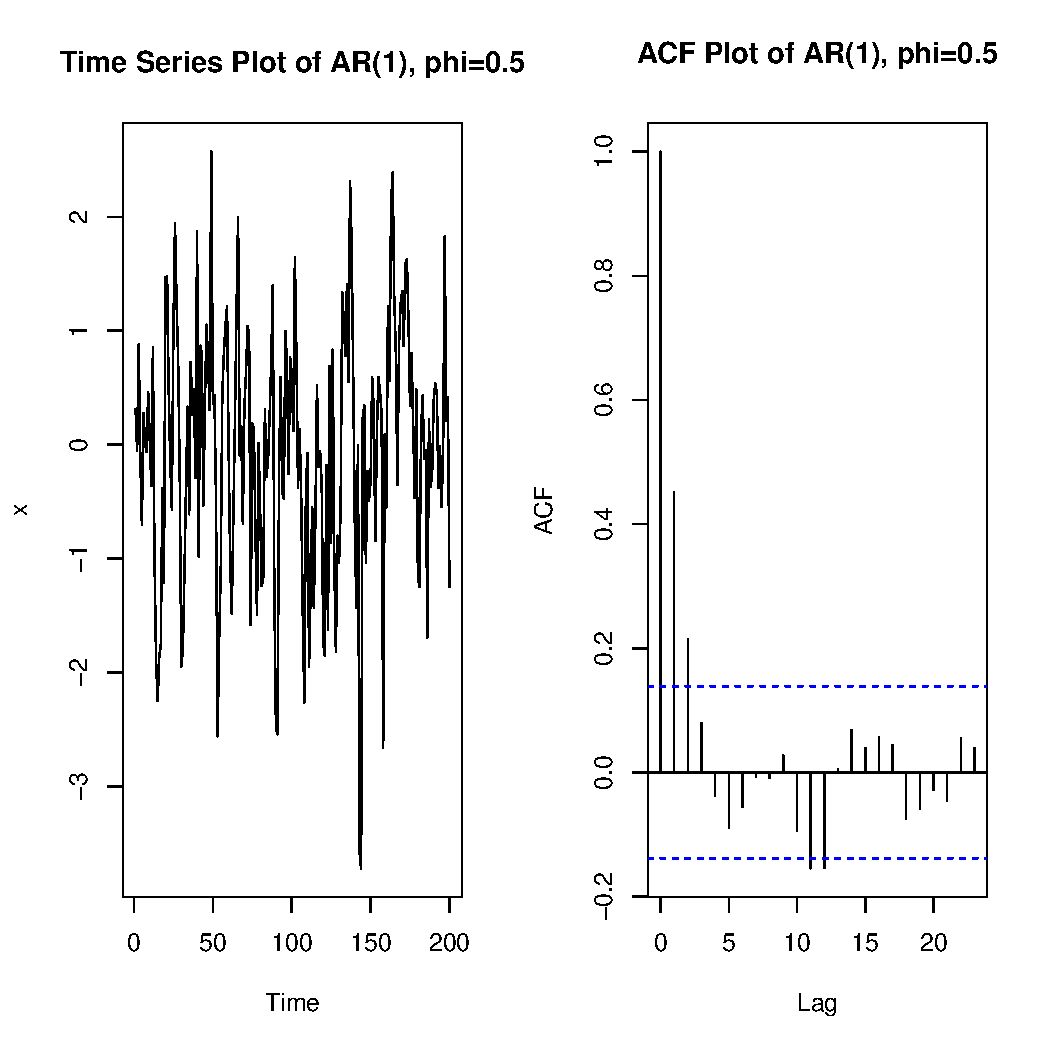
\includegraphics[width=110mm, height=80mm]{ar1s.pdf}

\end{frame}

\begin{frame}
\frametitle{Explosive AR(1)}

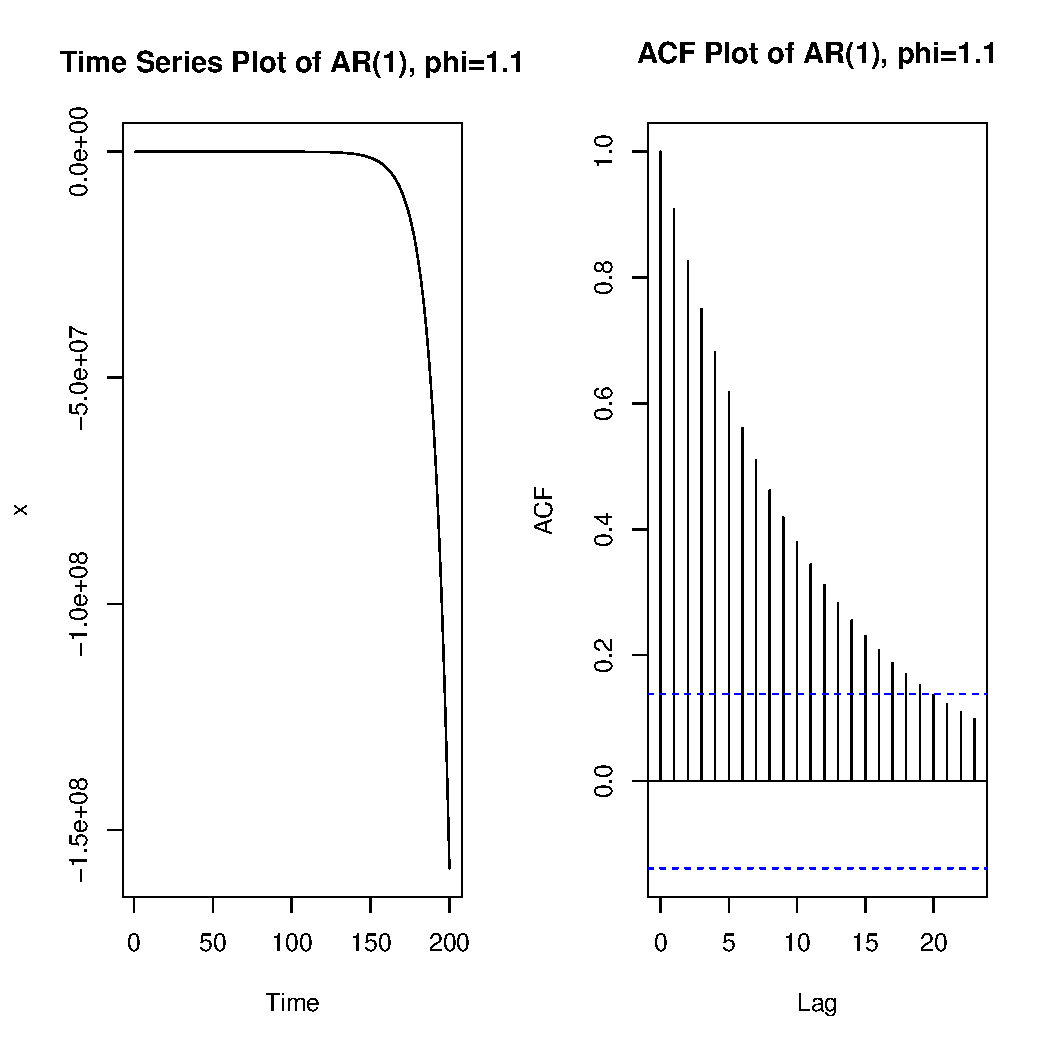
\includegraphics[width=110mm, height=80mm]{ar1ns.pdf}

\end{frame}

\begin{frame}
\frametitle{AR(1) and Causality}

We could rewrite the AR(1) process as
 $$
 x_t=\phi x_{t-1} + w_t  \Rightarrow x_{t-1} = \frac{1}{\phi} x_t - \frac{w_t}{\phi}
 $$
 and we have, by replacing the time index $t$ with $t+1$, $x_t =\phi^{-1} x_{t+1} - \phi^{-1} w_{t+1}$. Iterating this expression
forward, we have
 $$
 x_t=\phi^{-k} x_{t+k}-\sum_{j=1}^{k} \phi^{-j} w_{t+j}
 $$


\end{frame}

\begin{frame}
\frametitle{AR(1) and Causality}

Notice that if $|1/\phi|<1$, and taking the limit we obtain
 $$
 x_t=-\sum_{j=1}^{\infty} \phi^{-j} w_{t+j}.
 $$


\textbf{Question}: Why is such a model problematic?


\end{frame}

\begin{frame}
\frametitle{AR(1) and Causality}

For the AR(1) process, we require $|\phi|<1$ for causality. We will later extend and formalize a condition on the parameters $\phi_1, \phi_2, \cdots, \phi_p$ for an AR(p) process to be causal.


\end{frame}




\end{document} 